
%(BEGIN_QUESTION)
% Copyright 2006, Tony R. Kuphaldt, released under the Creative Commons Attribution License (v 1.0)
% This means you may do almost anything with this work of mine, so long as you give me proper credit

One challenge technicians face when calibrating low-pressure instruments is how to generate very low air pressures to simulate different low-pressure conditions for the pressure instrument under test.  Measuring low pressures is no problem at all: very simple manometers will do the job quite nicely.  Most mechanical air compressors, however, generate pressures far exceeding the range of most manometers.  Though it is possible to purchase precision pressure regulators for reducing such large pressures down to a level measurable by a manometer, these devices are expensive.

A simple way to ``divide'' the pressure output of a standard pressure regulator from a few PSI to a few inches of water is to use a pair of small valves (preferably needle valves allowing for precise adjustment) to throttle the flow of compressed air and vent the regulator's output to atmosphere, then tap between those valves to obtain a reduced pressure:

$$\includegraphics[width=15.5cm]{i00287x01.eps}$$

Complete the following schematic diagram showing an electrical model for this pneumatic system, and then explain how it works:

$$\includegraphics[width=15.5cm]{i00287x02.eps}$$

\underbar{file i00287}
%(END_QUESTION)





%(BEGIN_ANSWER)

$$\includegraphics[width=15.5cm]{i00287x03.eps}$$

I'll leave the explanation to you!

\vskip 10pt

Follow-up question \#1: explain what you could do with one or both of the two needle valves to {\it increase} the amount of pressure sent to the instrument under test.

\vskip 10pt

Follow-up question \#2: explain why placing a valve in ``series'' with the regulator's output will {\it not} adjust pressure to the instrument under test or the manometer.

$$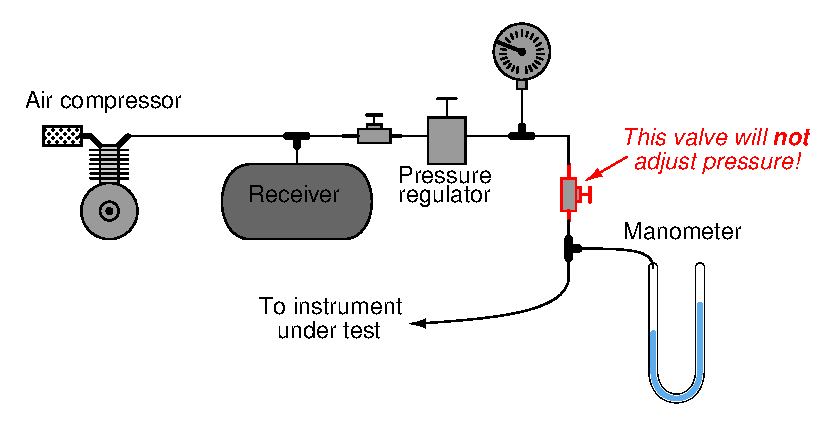
\includegraphics[width=15.5cm]{i00287x04.eps}$$

%(END_ANSWER)





%(BEGIN_NOTES)

The second follow-up question is particularly important, as novices often make this conceptual error.  They believe that placing a restriction between the pressure source and the instrument will somehow reduce the pressure going to that instrument.  In reality, it only {\it delays} changes in pressure to that instrument!  Just like a resistor placed in series with a voltmeter, a restriction cannot adjust pressure on its own where there is no flow.  As the instrument under test quite likely draws no air (it has infinite input impedance, to extend the electrical analogy), a series restriction will do nothing to reduce the pressure reaching it.

The delay comes from the volume of the tubing and of the instrument itself, acting as a capacitance to the series valve's resistance.  This forms an ``RC time constant'' with its characteristic first-order step response.

%INDEX% Calibration, generating low air pressures using a ``pressure divider'' network

%(END_NOTES)


